\documentclass[tikz,border=10pt]{standalone}
% Only base TikZ is needed; no extra libraries.
\begin{document}
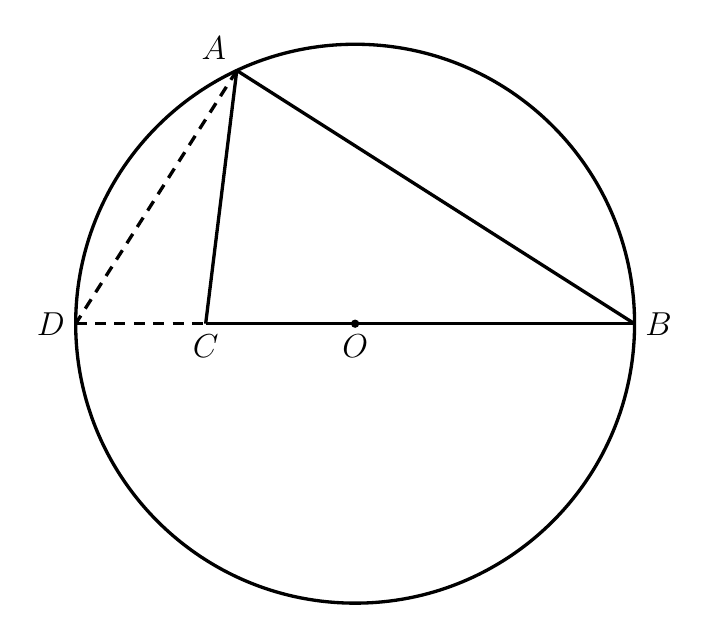
\begin{tikzpicture}[line width=1.2pt, line join=round]
  % Coordinates: O at origin, s = 0.015038 cm/px (STYLE METRICS scale)
  \coordinate (O) at (0,0);
  \coordinate (A) at (-1.503,3.216);   % px (204.09,63.49)
  \coordinate (B) at (3.548,0);        % px (539.94,277.08)
  \coordinate (C) at (-1.898,0);       % px (177.85,277.25)
  \coordinate (D) at (-3.549,0);       % px (68.01,277.52)

  % Circle centred at O, radius 236.03 px -- solid
  \draw[solid] (O) circle (3.549);

  % Solid C--B on the x-axis (through O)
  \draw[solid] (C) -- (B);
  % Dashed D--C on the x-axis
  \draw[dashed, dash pattern=on 4pt off 3pt] (D) -- (C);
  % Solid chords from A
  \draw[solid] (A) -- (B);
  \draw[solid] (A) -- (C);
  % Dashed A--D
  \draw[dashed, dash pattern=on 4pt off 3pt] (A) -- (D);

  % Small filled dot at O
  \fill (O) circle (1.5pt);

  % Labels
  \node[above left] at (A) {\fontsize{11.5}{13.8}\selectfont $A$};
  \node[right] at (B) {\fontsize{11.5}{13.8}\selectfont $B$};
  \node[below] at (C) {\fontsize{11.5}{13.8}\selectfont $C$};
  \node[left] at (D) {\fontsize{11.5}{13.8}\selectfont $D$};
  \node[below] at (O) {\fontsize{11.5}{13.8}\selectfont $O$};
\end{tikzpicture}
\end{document}